Le code suivant permet de tracer les graphes des fonction $\arccos$ et $\arcsin$, dans la figure~\ref{fig:ex_avance}.
% Code du fichier ex_avance.py
\begin{lstlisting}
import matplotlib.pyplot as plt
import math as m
from numpy import linspace

x1 = linspace(-1,1,200)
x2 = linspace(0,m.pi,200)
arccos = [m.acos(t) for t in x1]
cos = [m.cos(t) for t in x2]

plt.clf()
plt.plot(x1,arccos,color='b',label='$\\arccos(t)$', linewidth=2)
plt.plot(x2,cos,color='r',label='$\\cos(t)$', linewidth=2)
plt.plot([-0.5*m.pi,m.pi],[-0.5*m.pi,m.pi],color = 'g', 
  linestyle = '--', label = 'Première bissectrice du plan')
plt.xlabel('$t$')
plt.legend(loc=0)
plt.axes()
plt.savefig('ex_avance.png')
\end{lstlisting}

\begin{figure}[!h]
  \begin{center}
    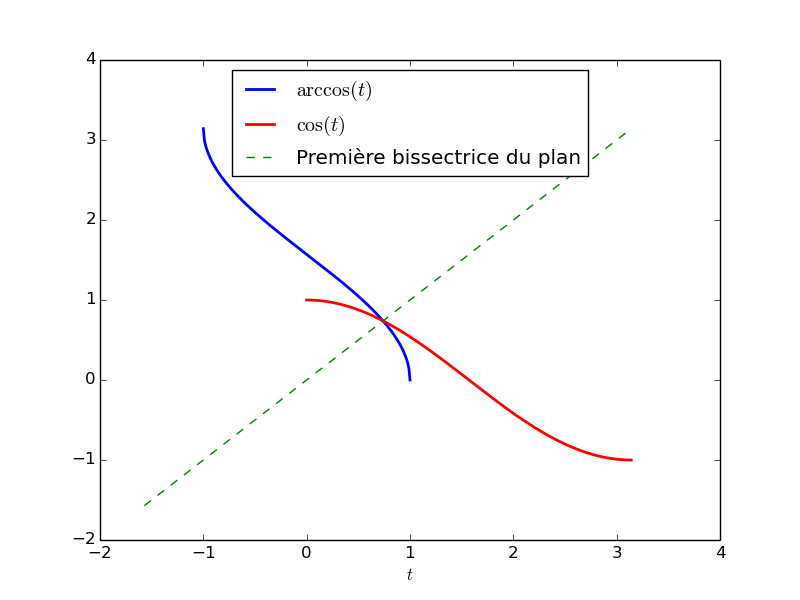
\includegraphics[scale = 0.7]{ex_avance}
    \caption{Graphes des fonctions $\arccos$ et $\cos$}
    \label{fig:ex_avance}
  \end{center}
\end{figure}  